\documentclass[a4paper,12pt,times,numbered]{template/PhDThesisPSnPDF}

\hypersetup{colorlinks=false}	% colour hyperlinks in default textcolour

\usepackage{subfig}		% multiple figures and caption in one figures

\usepackage[noabbrev]{cleveref}	% automatic selecting of reference type

\usepackage{colortbl}	% colour table cells
\usepackage{siunitx}		% SI units and alignment of decimals in tables
\usepackage{arydshln}	% dashed lines in tables

\usepackage{caption}		% setting caption width
\usepackage{nicefrac}	% fractions like 1/2

% sidecaptions on the right side with top alignment
\usepackage[rightcaption]{sidecap}
\sidecaptionvpos{figure}{t}

\usepackage{rotating}	% vertical text
\usepackage{pbox}		% used for linebreaks in table cell

%\usepackage{placeins}	% place all remaining floating elements

%\parskip 0em

%\renewcommand{\baselinestretch}{1.3} % one-and-a-half spacing
%\renewcommand{\baselinestretch}{1.6} % double spacing


\newtheorem{hypothesis}{Hypothesis}

% define metadata like author, title
% ************************ Thesis Information & Meta-data **********************
%% The title of the thesis
\title{Articulated Tracking for Humanoid Manipulation}
%\texorpdfstring is used for PDF metadata. Usage:
%\texorpdfstring{LaTeX_Version}{PDF Version (non-latex)} eg.,
%\texorpdfstring{$sigma$}{sigma}

%% Subtitle (Optional)
%\subtitle{Using the CUED template}

%% The full name of the author
\author{Christian Rauch}

%% Department (eg. Department of Engineering, Maths, Physics)
\dept{School of Informatics}

%% University and Crest
\university{University of Edinburgh}
% Crest minimum should be 30mm.
%\crest{\includegraphics[width=0.5\textwidth]{logo/UoE_Logo.eps}}
\crest{
\includegraphics[width=0.5\textwidth]{logo/uoe.eps}}
%% Use this crest, if you are using the college crest
%% Crest long miminum should be 65mm
%\crest{\includegraphics[width=0.45\textwidth]{University_Crest_Long}}

%% College shield [optional] 
% Crest minimum should be 30mm.
%\collegeshield{\includegraphics[width=0.2\textwidth]{CollegeShields/Kings}}


%% Supervisor (optional)
%% for multiple supervisors, append each supervisor with the \newline command
%\supervisor{\textbf{Prof. A.B. Supervisor\newline
%Prof. C.D. Supervisor\newline
%Prof. E.F. Supervisor\newline
%Prof. G.H. Supervisor}}

%% Supervisor Role (optional) - Supervisor (default) or advisor
% \supervisorrole{\textbf{Supervisors: }}
%% if no title is desired:
% \supervisorrole{}

%% Advisor (optional)
%% for multiple advisors, append each advisor with the \newline command
%\advisor{Advisor 1\newline
%Advisors 2\newline
%Advisor 3\newline
%Advisor 4}
     
%% Advisor Role (optional) - Advisor (default) or leave empty
% \advisorrole{Advisors: }
%% if no title is required
% \advisorrole{}


%% You can redefine the submission text:
% Default as per the University guidelines:
% ``This dissertation is submitted for the degree of''
%\renewcommand{\submissiontext}{change the default text here if needed}

%% Full title of the Degree
\degreetitle{Master of Science by Research}

%% College affiliation (optional)
%\college{King's College}

%% Submission date
% Default is set as {\monthname[\the\month]\space\the\year}
\degreedate{August 2016} 

%% Meta information
%\subject{LaTeX} \keywords{{LaTeX} {PhD Thesis} {Engineering} {University of
%Cambridge}}


% main document
\begin{document}

\frontmatter
\maketitle

\begin{declaration}

I declare that this thesis was composed by myself, that the work contained herein is my own except where explicitly stated otherwise in the text, and that this work has not been submitted for any other degree or processional qualification except as specified.

\end{declaration}
\begin{acknowledgements}      

First of all, I would like to thank my supervisor Dr. Maurice Fallon for his guidance throughout this thesis and for creating the working environment in which I could carry out my research. It is a pleasure for me to work with him and discuss research topics in the robot perception group.

Further, a special thanks goes to the postdoctoral researchers and Ph.D. students in the Valkyrie lab for helping me in getting the robot running and supporting me in my data collection.

I finally want to thank Julia for her unending patience during this period and for supporting me on my way.

\end{acknowledgements}
\begin{abstract}

Humanoid manipulator with several degree of freedom are versatile applicable to a variety of tasks by using man-made tools as opposed to task-specific manipulators. This comes with the cost of more complex control over the state of this manipulator and the tool.

This work addresses the problem of articulated manipulator and object tracking using visual feedback from the robot's own perception system. Current research has addressed different aspects of the problem like pose estimation of independent rigid parts, but only a few publications have addressed the specific case of manipulator and object tracking in the case where the state of the manipulator in respect to the observation frame is known.

The main contribution of this work is the investigation of the combined usage of visual perception and prior information from the reported manipulator state for a gradient based optimization approach.
This is motivated by the fact that gradient based approaches by design face the issue of local minimums in the objective function.

The evaluation of the gradient based approach using visual perception only, and using additional prior information, will on one side demonstrate the adverse effect of local minima for a manipulation task, and on the other side will show the benefits of exploiting prior information in the very same setting.
In this context, the work also addresses the issue of joint position encoder calibration as these values are the foundation of the exploited prior information.


\end{abstract}

\tableofcontents
\listoffigures
%\listoftables

\mainmatter

% chapters
\chapter{Introduction}

\section{Motivation}

Amongst all robot types, humanoid robots are one of the most versatile robots when it comes to acting in a world with man-made structures and tools. As such, they are a huge area of research involving multiple disciplines. Of special research interest is humanoid manipulation using hands that resemble human hands. Manipulators with several degree of freedom enables robots to reuse man-made tools to solve different kind of problems as opposed to be restricted to task-specific manipulators. Some of the tasks defined for the DARPA robotics challenge \cite{DRC2013} intended to advance robotic manipulation into this direction by setting a robot in a rescue scenario that involves the interaction with door handles (Door task), turning valves (Valve task), connecting a hose to a wye (Hose task) and using a drill to cut a hole in a wall (Wall task). Since the DRC rules stated that the robot needed to carry all of its manipulators during each trial, teams were force to use versatile manipulators.

The advantage of having such a generic manipulator comes with the costs of more complex control. Humanoid manipulation does not involve only the grasping of a tool but also the continuous control of this tool for the duration of the task. Since grasped tools are only indirectly connected to the robot's kinematic chain, additional perceptual information is needed to estimate and track the actual state of the manipulated object.


\section{Problem Definition and Research Aim}

Humanoid manipulation is a challenging task because of two main reasons: inaccurate forward kinematics and changing environment.
Inaccurate forward kinematics is mostly caused by improper calibrated joint encoders and linkage elasticity. Both issues can only be resolved to some extent by e.g. modelling joint position offsets \cite{Fallon2015} and stiffness coefficients \cite{Johnson2015}. The effect of inaccurate forward kinematics is visualised in \cref{fig:calibration_issue}.
By interacting with objects such as a valve, the robot needs to compensate the applied force by whole body control which likely changes the pose of the manipulated object in the camera frame.

\begin{figure}
\captionsetup{width=0.6\textwidth}
\centering
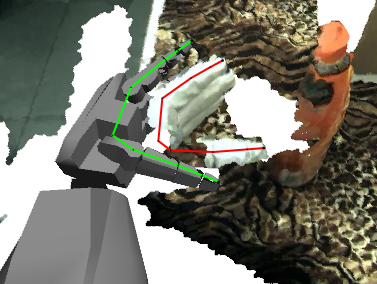
\includegraphics[width=0.5\textwidth]{images/valkyrie/joint_calibration_issue.png}
\caption{Joint calibration issue resulting in offset of reported pose (solid gray mesh, green marker) from perceived hand pose (coloured point cloud, red marker).}
\label{fig:calibration_issue}
\end{figure}

Both issues are in contrast with open loop industrial robot applications such as moving parts in a assembly line, where stiff actuators manipulate objects at defined poses. Using visual feedback to estimate the configuration of the manipulator and the pose of the manipulated object could be the key step to enable closed-loop manipulation.
In return, visual tracking of highly articulated manipulators and objects causes interesting research questions itself again.

\paragraph{Manipulator tracking}
The main problem of tracking highly articulated manipulators with several degree of freedom is the large variety of their appearance. Using classical object detection methods on this problem would require an enormous training set of different configurations at different lighting conditions. In addition, classification results must be provided at real-time. On one side, the problem can be simplified in the context where a robot is observing its own manipulator by using a robot model representation and its joint encoder values. On the other side, the before mentioned issue of inaccurate forward kinematics reduces the value of these encoder values.

The \emph{primary aim} of this thesis is investigating the effect of using visual perception and reported joint encoder values in conjunction to enable tracking if either of the two information is not available or inaccurate.

\paragraph{Object tracking}
In contrast to the manipulator, we usually have no prior information about the pose of the object up to the point where the manipulator gets in contact with the object. The Amazon Picking Challenge 2015 \cite{Correll2016} showed that detection and tracking of ordinary consumer objects is still a challenging task. Amongst the 25 products used in the challenge were objects of varying appearance (e.g. non rigid objects), objects with meshed material (such as bins) and objects with reflective and translucent material. Classical machine learning approaches that rely on descriptive keypoint features such as SIFT fail in cases where textual information is not available either because of lighting conditions or material properties.

The \emph{secondary aim} of this thesis is the investigation of object tracking with lack of texture.

\chapter{Related Work}
\label{sec:related_work}

This chapter is based on a previous literature review and research proposal that lead to this thesis. It has been extended by recent publications and a clarification where this work contributes to the current state of the art.


\section{Sensor Modalities}

\subsection{2D Vision}
Early work in this area has been limited to single 2D perception capabilities. Thus, a common approach was to project known 3D objects into 2D and to compare these with perceived data from images. Chliveros et al. \cite{Chliveros2013}, Teuli\`ere et al. \cite{Teuliere2010}, Choi et al. \cite{Choi2012} and Azad et al. \cite{Azad2011} rely on an exact 3D model of an object for tracking and use a particle filter to maintain multiple hypotheses of the object's pose. These hypotheses are projected into a 2D plane (prediction step) and evaluated at the observation step. At this observation stage, the predicted edges of the 3D model in the 2D plane are compared with the linear edges and shapes extracted from the actual 2D sensor data. As a positive aspect, these approaches do not require range sensors but they do require detailed knowledge of the object's dimensions beforehand and do not exploit features from colour or texture, excluding Choi et al. which uses SIFT keypoints as initial pose estimation.

Recent template matching approaches explore special properties of boundary edges. Mu\~nos et al. \cite{Munoz2016} for example use HOG features (histograms of oriented gradients) to find corresponding edges between the template and the image. Cao et al. \cite{Cao2016} on the other side argue that HOG features lose pixel-level detail and instead use the cross-correlation between the Laplacian of Gaussian between templates and image patch. All template matching approaches have in common that they require a large database with templates of objects in all expected views.

\subsection{3D Vision}
\label{sec:3d_vision}

\paragraph{Single Articulated Objects}
With the advancement in range sensing and especially the availability of consumer depth sensors like the Kinect, similar approaches have been extended to 3D perception. Krull et al. \cite{Krull2015} apply a particle filter to estimate the object's pose in single images using RGB-D data by maintaining multiple hypotheses of the object pose. The observation distribution is generated from a discriminative learning method. Using example objects and an example background image, a random forest automatically learns useful features from the RGB-D data during a training phase. Once trained, the probability distribution of object class and coordinate location within the object is obtained for each new image.
%Their motion model assumes that an object continues its current motion and only changes by normally distributed translation and rotation.

The work of Shotton et al. \cite{Shotton2013} deals with complete body pose estimation and tracking of body parts. Instead of maintaining pose hypotheses of a single object, complete human skeleton hypotheses are evaluated. The observation distribution is generated by a discriminative classifier (random forest) using depth features for classifying 31 body parts. To achieve robustness and flexibility with their approach, a massive amount of training data is synthetically generated by rendering a body mesh at different sizes and with different joint configurations using motion capture.
The same combination of random forests and primitive depth features is applied by Widmaier et al. \cite{Widmaier2016} in a robotic manipulator context. However, they skip the intermediate task of classifying parts of the robot and instead predict its joint configuration directly.

A similar discriminative approach is used by Sharp et al. \cite{Sharp2015} to track articulated human hands.
For reinitialisation after tracking loss, the hierarchical distribution of hand poses is learned by a discriminative approach using synthetically generated training data.
Synthetic depth images are generated by sampling from a prior distribution of global hand translation and rotations, realistic wrist poses and six predefined finger and thumb states.
For finding the optimal hand configuration, they apply a mixture of particle swarm optimization (PSO) and genetic algorithms. In particle swarm optimization, particles represent solutions in the search space whose state is updated by the particle's own best known solution and by the swarm's global best known solution. PSO does not require the gradient of the optimized function.
Particles in PSO represent hypotheses as in particle filters, but their state is updated such that at least one particle's state is the global solution, whereas the current global solution of a particle filter is the expectation of the probability distribution formed by all particles (Monte Carlo expectation estimation).
At tracking loss, these hypotheses are reinitialized by the prediction of the discriminative method on the new depth input.
Each hypothesis of the particle swarm is evaluated by rendering its state and comparing it with the actual perceived sensor input.
To form the next generation of the particle swarm, particles with bad hypotheses are randomized and re-initialized.

\paragraph{Combined Object and Manipulator Tracking}
Pauwels et al. \cite{Pauwels2015} combined pose detection for reinitialization with pose tracking using dense motion and the information from depth data and colour. They rely on sparse SIFT keypoints sampled at equidistant viewpoints to obtain initial pose estimates and to reinitialize the tracker in case of tracking loss. The poses are continuously estimated using the shape and dense motion estimates of the object. This combination of both estimates enables them to cover difficult cases where the objected is blurred by motion or occluded (\cref{fig:simtrack_poses}).
The motion is represented as the optical flow on raw image data and on images which are augmented by objects rendered at their current estimated state.

\begin{figure}[h]
\centering
\subfloat[]{\includegraphics[width=0.33\textwidth]{images/related_work/dense_pose1.png} }
\subfloat[]{\includegraphics[width=0.33\textwidth]{images/related_work/dense_pose2.png} }
\subfloat[]{\includegraphics[width=0.33\textwidth]{images/related_work/sparse_pose1.png} }
\caption[SimTrack object tracking]{SimTrack: Examples of correct classified object poses. (a) and (b) using \textit{dense} estimation for small and blurry observations, (c) using \textit{sparse} keypoints for occluded observations. (Source: \cite{Pauwels2015}, figure 13)}
\label{fig:simtrack_poses}
\end{figure}

The multi-object tracking in SimTrack was extended for articulated objects \cite{Pauwels2014} by incorporating the pose updates into a kinematic chain with constraints. The pose of each rigid part is estimated independently from each other. The links between parts can be constrained to define free and static joints. The complete update of the kinematic chain takes into account the individual pose updates per part and the movement constraints of parts to each other.

SimTrack was further extended for joint object and manipulator tracking \cite{Pauwels2014b}, where the manipulator (arm and hand) is considered rigid after the joint values are used to articulate the model. As the approach relies on inaccurate joint encoder values, only the hand (which is assumed to be rigidly connected to the object) is tracked. Further, because the robot's surface is low textured, sparse features cannot be exploited.

The DART framework presented by Schmidt et al. \cite{Schmidt2015, Schmidt2015b} aims to provide a general framework for articulated tracking using depth sensors. DART assumes that the articulated model is given as a set of rigid objects with transformation from the kinematic chain and a local signed distance function that gives the distance of a point to the hull of the object (and is negative inside). The optimal joint configuration that minimizes the distance of the model to the observed point cloud is recovered by a gradient based optimization approach. \Cref{fig:dart_justin_est} shows this exemplary for hands and an object in a bimanual manipulation task.
Compared to particle filters, this does not maintain explicit hypotheses but optimizes on the distances.

\begin{figure}[h]
\centering
\includegraphics[width=0.5\textwidth]{images/related_work/dart_estim.png}
\caption[DART manipulator tracking]{DART: Depth based estimation of robot configuration projected on top of the perceived RGB image. (Source: \cite{Schmidt2015b}, figure 2)}
\label{fig:dart_justin_est}
\end{figure}

\subsection{Contact Sensors}

Schmidt et al. \cite{Schmidt2015b} and Koval et al. \cite{Koval2015} showed that contact sensing can be used to estimate the pose of an object or to reject visually proposed poses.
Koval et al. \cite{Koval2015} manipulated an object by pushing it over a planar surface and estimated its 2D position on the surface and orientation solely by contact sensors. They restrict their sensing to 9 strain gauges on the fingers and the palm of the hand, which only provides boolean information about contact (contact or no contact). By enhancing a particle filter to prevent particle starvation caused by the discrete states of the observation, they are able to estimate the position and orientation despite the low dimensionality of sensing.

As this approach does not scale from 3 DOF (2D position + 1D rotation) to 6DOF poses in 3D, contact sensing is best applied in conjunction with other sensing to eliminate unlikely hypotheses as in \cite{Schmidt2015b}.

\subsection{Kinematics and Constraints}

The work of Schmidt et al. in \cite{Schmidt2015} is extended in \cite{Schmidt2015b} to incorporate physical constraints, namely intersection of the manipulator with the object and contact with the object.
If the manipulated object is rigidly connected to a manipulator, the joint encoder values can be an important source to improve the object's pose estimate.

On the other hand, kinematic chains can be used to constrain estimated configurations to physically reasonable and likely values and eliminate unlikely hypotheses \cite{Shotton2013, Sharp2015}.
Whereas physical constraints are fixed, e.g. they always hold, kinematic constraints are soft, e.g. unlikely and unreasonable states might still occur.

\section{Real-Time Capabilities}

All of the particle filtering based approaches trade off the quality of the resulting pose estimation, as represented by the particles, with real-time constraints. An increasing number of particles cover a wider range of pose hypotheses but also increase the computation time.

Krull et al. \cite{Krull2015} however showed, that using a good proposal distribution can reduce the required amount of particles to achieve similar results compared to particle filters using generic distributions with many more particles.

A general and common solution to meet real-time constraints is the parallelisation of algorithms and offloading of computations to GPUs. Exemplary, the independent state updates for particles in a particle filter \cite{Choi2013} or the independent lookup of shortest distances of points to multiple models \cite{Schmidt2015} can easily be parallelized.


\section{Model-based and Model-free}

Tracking of rigid or articulated objects usually requires knowledge of the dimensions of the object or the manipulator beforehand. In contrast, there exist approaches that model manipulated objects and kinematic chains online during manipulation.

Krainin et al. \cite{Krainin2011} modelled objects online by tracking the manipulator and the object at the same time during a grasping task.
They address the issue of relying solely on either the object's appearance or the manipulator's joint values. Using only a single source of information can cause ambiguous and incorrect pose estimates for textureless and symmetric objects with lack of visual distinctive features.
By using multiple sources of information they are able to map highly symmetric 3D objects with lack of visual features and in presence of noisy joint values.

The issue of faulty or absent of joint encoder values is addressed by Sturm et al. \cite{Sturm2009}. In their work, the kinematic chain of an arm is learned from scratch and enables adaptation in cases of malfunction, e.g. if a joint is blocked or its strength decreases over time.
Si et al. \cite{Si2013} learn the variety of appearance of articulated objects as a hierarchical composition of parts as AND and OR nodes without providing labels. AND nodes define connection of parts, e.g. torso and limbs, and OR nodes represent different configurations of the same part. As a result, they can provide generic configurable templates for articulated objects.

The availability of accurate CAD models of robots and large online databases of 3D objects \cite{Firman2016, Singh2014} reduces the need to create models of common objects and enables the generation of huge synthetic training sets for discriminative approaches.

\section{Features}
Discriminative approaches, that learn the appearance of parts \cite{Shotton2013, Krull2015, Pauwels2015} or complete poses \cite{Sharp2015}, rely on manually designed features or keypoints like edges, SIFT \cite{Pauwels2015, Morwald2010} or depth features. In the RGB-D domain, where these features often neglect one of the channels, exploiting all the information is beneficial. Ren et al. \cite{Ren2012} applied kernel descriptor for RGB-D scene labelling and showed superior performance of RGB-D descriptors compared to RGB or depth only descriptors.

\paragraph{RGB-D Features and Descriptors}
Learned features not only provide a way to classify 3D objects by machine learning algorithms (e.g. SVM), but also provide interest points for pose estimation by homography.

Gupta et al. \cite{Gupta2014} combined feature learning on RGB-D data with pixel-wise classification for segmenting objects in depth data. Object region proposals from contours are classified by a linear SVM using RGB-D features learned by a Region-based Convolutional Neural Net (R-CNN). Classified regions are separated in foreground and background pixels using random forest and low-level features such as the pixel coordinate and depth, distance to ground plane and gravity vector. The foreground pixels are allocated to superpixel and classified into one of the many categories.

Blum et al. \cite{Blum2012} demonstrated an approach that learns RGB-D features in an unsupervised manner by convolutional k-means (CKM) around SURF interest points. Similar performance can be achieved by the hierarchical matching pursuit (HMP) approach \cite{Bo2013} in classification tasks. It was shown that HMP is applicable for pose estimation, achieving appropriable results for weak-symmetrical objects with unambiguous viewpoints.

\paragraph{Joint Detection}
In the work of Jain et al. \cite{Jain2015}, the location of joints in 2D image sequences are learned from labelled raw image data using a convolutional neural network (CNN) by only providing simple motion features. These positions can be used to infer a kinematic model of articulated objects.

Tompson et al. \cite{Tompson2014} applied a CNN to joint detection using depth data and are able to estimate the location of occluded parts without the need to provide joint connectivities from a kinematic model. They state that the inference of occluded parts is especially enabled by the hierarchical compound features learned in the CNN.

The spatial relation of compound parts is also exploited by Jiu et al. \cite{Jiu2014}. By learning a pixel-wise segmentation of human body parts incorporating spatial relation, the classification performance is increased with no additional computation costs during testing phase. As with most deep learning applications, they learn from raw depth data and do not require precomputed features.



\section{Conclusion from State-of-the-Art}
\label{sec:discussion}

The majority of the presented work in the field of articulated tracking applies a discriminative approach to depth sensor data. Because of the high variance in shape and viewpoint of the tracked objects, a very large amount of training data is required to learn a sufficient distribution of articulations. If the articulated objects are known beforehand and a large variety of sensor data is available or can be generated, this is a promising approach.

However, relying solely on either the learned representation of objects or the kinematics of the manipulator fails in cases of low structured objects (highly symmetric, lack of texture and visual features), non-reliable sensor data (occlusions, reflection of sunlight, shadows in depth data, non-IR-reflective surfaces) and noisy or improper calibrated joint encoders.

Tracking and pose estimation of multiple objects is only considered in a small fraction of the presented work. Most of the presented work focuses either on the tracking of rigid objects or the tracking of manipulators; or assumes no interaction of tracked objects.

This thesis contributes towards the optimal integration of prior information from joint position sensing in a setting where a robot is visually observing its own manipulator. We base our work on the optimization approach presented by Schmidt et al. \cite{Schmidt2015}, that in its original implementation uses solely depth observations to find an optimal robot configuration.

\chapter{Methods}

\section{Gauss-Newton Algorithm}

The \textit{Gauss-Newton} algorithm is a method for finding the optimal set of parameters $\mathbf{p}$ that minimizes the sum of squares of non-linear vector-valued objective functions $e(\cdot)$
%
\begin{equation}
\hat{\mathbf{p}} = \arg\min_{p} \sum_{i=1}^N\left[ e_i(\mathbf{p})^2\right] .
\end{equation}

The Gauss-Newton algorithm is derived from the \textit{Newton} algorithm for finding roots and extremal points which itself is based on the Taylor series expansion. The Newton method for finding extremal points of the scalar objective function $f(x)$ is an iterative procedure
%
\begin{equation}
x_{t+1} = x_t - \frac{f^{(1)}(x_t)}{f^{(2)}(x_t)}
\label{eqn:newton_minimum}
\end{equation}
%
starting at an initial state $x_0$ using the first- and second-order derivatives ($f^{(1)}$, $f^{(2)}$) of the objective function.

For finding the minimum of the function $e(\cdot)$ with respect to a parameter vector $\mathbf{p}$, the first- and second-order partial derivatives are used. In particular, the first- and second-order derivatives in \ref{eqn:newton_minimum} are replaced by the gradient $\nabla e(\mathbf{p})$ and the Hessian $\nabla^2 e(\mathbf{p})$ of the objective function $e$.
The partial derivatives of the vector-valued function $e(\cdot)$ with respect to the parameter vector $\mathbf{p}$ are aggregated in the \textit{Jacobian} matrix $J\in \mathbb{R}^{i \times j}$ with elements
%
\begin{equation}
J_{i,j} = \frac{\partial e_i(\mathbf{p})}{\partial p_j} .
\end{equation}
%
Hence,
\begin{align}
\nabla e(\mathbf{p}) &= J^\top e(\mathbf{p}) \\
H(e) = \nabla^2 e(\mathbf{p}) &= J^\top J +  \sum_{i=1} e_i(\mathbf{p}) \nabla^2 e_i(\mathbf{p}) .
\end{align}

For small $e$, the Hessian $H(e)$ can be approximated by
\begin{equation}
H(e) \approx J^\top J
\end{equation}
%
neglecting the second-order derivatives. This approximation is used in the Gauss-Newton algorithm and the parameter update step becomes
%
\begin{align}
\mathbf{p}_{t+1} &= \mathbf{p}_{t} - \Delta\mathbf{p} \\
&= \mathbf{p}_{t} - H(e)^{-1} \cdot \nabla e(\mathbf{p}) \\
&= \mathbf{p}_{t} - \left(J^\top J\right)^{-1} \cdot J^\top e(\mathbf{p}) .
\end{align}

The parameter update $\Delta\mathbf{p}$ is proportionally driven by the gradient of the objective function and inverse proportional by the approximation of the Hessian.

\chapter{Evaluation}

\section{Effect of Prior Information}

This section will evaluate the application of prior information in a setting where a robot hand moves close to an object and a table. Two sources of depth information will be considered: enhanced stereo matching using IR dot patterns (denoted as \emph{stereo}) and structured light (denoted as \emph{xtion} as in Asus Xtion).

\subsection{Hypotheses}

In the base implementation of the assessed tracking approach, its gradient is mainly determined by the signed distance function. Hence, the optimization is mainly driven by the observation once the iteration is initialized with the reported state. Using additional information that effects the gradient can improve the state estimation by driving it away from distracting observations.

%The deviation of the estimated to the reported robot state is measured in joint and task space. Hence, the error is defined as measurements of the reported pose minus measurements of the estimated pose.

\begin{hypothesis}(Distracting sensor readings)\\
Distracting sensor readings will impair the tracking performance of the manipulator.
\end{hypothesis}

\begin{hypothesis}(Use of prior information)\\
Using prior information will reduce the negative effects of distracting sensor readings. Further, increasing weights will enhance this effect.
\end{hypothesis}


\subsection{Setup}

A robot is placed in front of a table with a bottle on it. The left hand is moving from close to the table plane towards the object. Once the object is pushed, the hand moves up and back to its initial position.
\Cref{fig:prior_setting} shows the setup with stereo depth and reported robot configuration at the initial state.
The motion sequence is divided into 5 states which change by 4 movements. The movement phases are defined in \cref{tab:prior_movement_phases}. The first three states and the final state are shown in \cref{fig:prior_movement_phases}.
Especially the movement phases 2 and 4, respectively movements starting in states shown in \cref{fig:prior_movement_phases_start,fig:prior_movement_phases_start} are of interest.

\begin{figure}
\centering
\begin{minipage}{0.45\textwidth}
\centering
\includegraphics[width=1.0\textwidth]{images/eval_prior/sequence/prior_setting.png} 
\caption{Setup}
\label{fig:prior_setting}
\end{minipage}
%
\hspace{0.3cm}
\begin{minipage}{0.45\textwidth}
\vspace{0.8cm}
\centering
\subfloat[start (t=0)]{\includegraphics[width=0.5\textwidth]{images/eval_prior/sequence/bottle_0_init.png} \label{fig:prior_movement_phases_start}}
\subfloat[moved upwards (t=10)]{\includegraphics[width=0.5\textwidth]{images/eval_prior/sequence/bottle_10_up.png} }

\subfloat[object contact (t=22)]{\includegraphics[width=0.5\textwidth]{images/eval_prior/sequence/bottle_22_object.png} 
\label{fig:prior_movement_phases_contact}}
\subfloat[end (t=35)]{\includegraphics[width=0.5\textwidth]{images/eval_prior/sequence/bottle_35_end.png} }
\caption{Sequence of states between movements}
\label{fig:prior_movement_phases}
\end{minipage}
\end{figure}

\begin{table}
\centering
\begin{tabular}{|c|l|l|}
\hline
 & \emph{time (s)} & \emph{movement description} \\
\hline
1 & 0$\dots$3 & arm resting on table \\
\hline
2 & 3$\dots$10 & upward from table \\
\hline
3 & 10$\dots$20 & towards object \\
\hline
4 & 20$\dots$30 & away from object \\
\hline
5 & 30$\dots$35 & downward towards table \\
\hline
\end{tabular}
\caption{Phases of arm movement}
\label{tab:prior_movement_phases}
\end{table}

During the movement, depth data is collected simultaneously from the MultiSense stereo sensor and the Asus Xtion structured light sensor. Hence, the stereo feature matching benefits from the distinctive IR dots.

\subsection{Results}

The error in joint and task space is computed as L2 norm (Euclidean distance) of its components and plotted over time. In joint space these components are the left fingers (13 DoF: 3 \emph{leftIndexFingerPitch}, 3 \emph{leftMiddleFingerPitch}, 3 \emph{leftPinkyPitch}, 3 \emph{leftThumbPitch} and 1 \emph{leftThumbRoll}) and the left arm (7 DoF: \emph{leftShoulderPitch/Roll/Yaw}, \emph{leftElbowPitch}, \emph{leftForearmYaw}, \emph{leftWristRoll/Pitch}). In task space, the 3D position ($x,y,z$) and the 3D orientation (\textit{roll}, \textit{pitch}, \textit{yaw}) of the left hand (frame: \emph{leftPalm}) are computed via FK on the reported and estimated robot configuration.

\subsubsection{Common Weight}

The plots compare the joint and task space errors for the two depth sources for common weights in the range 0 to 5. The common weighting scheme \emph{Weighted L2 norm of joint position deviation} (objective function \cref{eqn:objf_weightedL2}) is applied. A weight of 0 indicates that no prior is used at all.

\paragraph{Stereo}

\Cref{fig:stereo_joint_error} compares the joint error for left fingers and arm. For both parts, after the optimization reaches the steady state, the maximum error is reached when no prior information from the reported configuration is used.
The general trend is that the error decreases with increasing weight. This is not true for the arm movement in the second half of phase 4 ($t=[20,30]$), where weights of $0.2$ and $0.5$ result in larger errors than using no prior.

The largest decrease in error can be seen for the finger joints when using already a small weight of $0.2$. A similar effect is not present for the arm joints. This is presumably because the robot can only observe the lower part of its arm and hence the arm configuration is mostly determined by its initial state close to the reported state.


\begin{figure}
\centering
\subfloat[finger joints]{\includegraphics[width=0.5\textwidth]{images/eval_prior/common_weights/stereo_finger_joint_error.pdf} \label{fig:stereo_joint_error_hand} }
%
\subfloat[arm joints]{\includegraphics[width=0.5\textwidth]{images/eval_prior/common_weights/stereo_arm_joint_error.pdf} \label{fig:stereo_joint_error_arm} }
\caption{Stereo, joint space error for left finger and arm joints}
\label{fig:stereo_joint_error}
\end{figure}

As the hand position and orientation only depends on the arm configuration but not the finger configuration, we expect some relation between the joint error of the arm and the pose error on the hand frame. We can see this relation, when comparing the joint space error for the arm in \cref{fig:stereo_joint_error_arm} and the hand pose error in \cref{fig:stereo_hand_pose_error}. In particular the error increases in phases where the hand moves upwards and when it moves away from the object. The position error can be reduced significantly when using a prior with low weight ($0.2$), where as the orientation error reduces only when using prior weights larger or equal than $0.8$.

\begin{figure}
\centering
\subfloat[position error]{\includegraphics[width=0.5\textwidth]{images/eval_prior/common_weights/stereo_hand_pos_error.pdf} \label{fig:stereo_hand_pos_error}}
%
\subfloat[orientation error]{\includegraphics[width=0.5\textwidth]{images/eval_prior/common_weights/stereo_hand_ori_error.pdf}
\label{fig:stereo_hand_ori_error}}
\caption{Stereo, task space error for left hand pose}
\label{fig:stereo_hand_pose_error}
\end{figure}



\paragraph{Asus Xtion}

Using the structured light sensor Asus Xtion, the behaviour of decreasing error with increasing weight is comparable to that one saw for the stereo matching sensor. Similar to the stereo sensor (\cref{fig:stereo_joint_error_hand}), the error on the finger joints reduces significantly when already using a small weight of $0.2$ (\cref{fig:xtion_joint_error_hand}).
In contrast to small the error on the arm joints when using stereo in the phase of moving towards the object (\cref{fig:stereo_joint_error_arm}), the error in this phase when using the Xtion sensor is fairly large for no and low weighted prior (\cref{fig:xtion_joint_error_arm}).

\begin{figure}
\centering
\subfloat[finger joints]{\includegraphics[width=0.5\textwidth]{images/eval_prior/common_weights/xtion_finger_joint_error.pdf} \label{fig:xtion_joint_error_hand}}
%
\subfloat[arm joints]{\includegraphics[width=0.5\textwidth]{images/eval_prior/common_weights/xtion_arm_joint_error.pdf} \label{fig:xtion_joint_error_arm}}
\caption{Xtion, joint space error for left finger and arm joints}
\label{fig:xtion_joint_error}
\end{figure}

As before, the hand pose error is only effected by the arm joint errors and thus the hand position error shown in \cref{fig:xtion_hand_pos_error} is large in the same moving phase towards the object. For using the structured light sensor, a common weight of at least $2$ is required to drive the solution towards the reported hand position.

\begin{figure}
\centering
\subfloat[position error]{\includegraphics[width=0.5\textwidth]{images/eval_prior/common_weights/xtion_hand_pos_error.pdf} \label{fig:xtion_hand_pos_error}}
%
\subfloat[orientation error]{\includegraphics[width=0.5\textwidth]{images/eval_prior/common_weights/xtion_hand_ori_error.pdf} \label{fig:xtion_hand_ori_error}}
\caption{Xtion, task space error for left hand pose}
\label{fig:xtion_hand_pose_error}
\end{figure}

\subsubsection{Individual Weights}

Individual weighting is applied to stereo depth data only. This weighting scheme enables to weight each combination of joint derivations separately as defined by \cref{eqn:objf_indiv_weighted}. For simplicity, only single joint deviations are weighted. That is, the weight matrix $Q$ will be a diagonal matrix where only the diagonal elements $q_{i,i}$ will be changed.

In this scenario, three setting of joints are weighted and this scheme is captured in the legend as follows: first, all diagonal elements of $Q$ are set to the weight \emph{q}, second, the 13 finger joints are set to the weight \emph{fingers} and optionally third, the two palm joints (leftWristRoll, leftWristPitch) are set to the value \emph{parm}. E.g., a plot named \texttt{q 1, fingers 0.2, palm 5} indicates that finger joints in the diagonal are weighted by $0.2$, palm joints are weighted with $5$ and the remaining joints are weighted with $1$.

\Cref{fig:indiv_joint_error} shows again the joint space error for fingers and arms separately. From these plots we can see that the individual weighting affects the fingers and the arm in different ways. The finger joint error in \cref{fig:indiv_joint_error_hand} shows that, raising the palm weights and keeping the remaining constant actually impairs the performance (e.g., compare constant \texttt{q 1, fingers 0.2} and palm weights raised to \texttt{palm 5}). In contrast to this, the arm joint error is reduced when increasing the palm weights and keeping remaining weights constant (e.g., compare constant \texttt{q 0.2, fingers 0.2, palm 5} and palm weights raised to \texttt{q 0.2, fingers 0.2, palm 25}).

\begin{figure}
\centering
\subfloat[finger joints]{\includegraphics[width=0.5\textwidth]{images/eval_prior/inidv_weights/stereo_finger_joint_error.pdf} \label{fig:indiv_joint_error_hand}}
%
\subfloat[arm joints]{\includegraphics[width=0.5\textwidth]{images/eval_prior/inidv_weights/stereo_arm_joint_error.pdf} \label{fig:indiv_joint_error_arm}}

\caption{Joint space error for individual weighting}
\label{fig:indiv_joint_error}
\end{figure}

Again, the arm joints directly influence the pose error of the hand as seen in \cref{fig:indiv_pose_error}. \Cref{fig:indiv_hand_pos_error} shows that the hand position mostly benefits from using some weight $>1$ on the palm joints whereas weighting the remaining joints does not contribute to driving the solution towards the reported hand position. For the hand orientation error in \cref{fig:indiv_hand_ori_error}, the error is usually reduced if the weights on the palm joints are increased (e.g. $1$ to $5$, or $5$ to $25$) and remaining joints keep their weights. We can also see that using small weights ($q=0.2$) for all joints but the palm actually results in a estimated position closer to the reported position than what is achieved by larger weights ($q=1$).

\begin{figure}
\centering
\subfloat[]{\includegraphics[width=0.5\textwidth]{images/eval_prior/inidv_weights/stereo_hand_pos_error.pdf} \label{fig:indiv_hand_pos_error}}
%
\subfloat[]{\includegraphics[width=0.5\textwidth]{images/eval_prior/inidv_weights/stereo_hand_ori_error.pdf} \label{fig:indiv_hand_ori_error}}

\caption{Task space error for individual weighting}
\label{fig:indiv_pose_error}
\end{figure}

\subsubsection{Object Position}

Most of the time, the pose of the object (bottle) is mainly affected by the optimization. Only when there is interaction between the manipulator and the object, it gets indirectly dependant on the joint values and hence the prior weight. The object's pose is initialise close to the true observed state and is expected to not move until the end of the reaching phase. \Cref{fig:bottle_movement} compares the object's distance to the image origin for stereo and xtion datasets and gives an indication about its movement. The bottle in the stereo data (\cref{fig:bottle_movement_stereo}) stays, as expected, close to its initial position until the end of the reaching phase. In contrast, the bottle in the Xtion dataset (\cref{fig:bottle_movement_xtion}) already moves at the beginning to its final pose.

\begin{figure}
\centering
\subfloat[stereo]{\includegraphics[width=0.5\textwidth]{images/eval_prior/stereo_obj_pos.pdf} \label{fig:bottle_movement_stereo}}
\subfloat[xtion]{\includegraphics[width=0.5\textwidth]{images/eval_prior/xtion_obj_pos.pdf} \label{fig:bottle_movement_xtion}}
\caption{Movement of bottle during robot arm movement}
\label{fig:bottle_movement}
\end{figure}

A snapshot of the perceived point cloud is depicted in \cref{fig:bottle_point_cloud} for a state at the beginning of the experiment for both depth sources. A comparison of these sources show that: 1) the stereo depth source contains data with larger depth, and 2) the stereo depth source also contains more points of the object than the structured light sensor. It must be noted that the structured light sensor is mounted above the stereo sensor pointing into the same region of interest. It thus perceives the scene at a steeper angle.

\begin{figure}
\centering
\subfloat[stereo point cloud]{\includegraphics[width=0.4\textwidth]{images/eval_prior/stereo_bottle.png} }
\hspace{1cm}
\subfloat[xtion point cloud]{\includegraphics[width=0.4\textwidth]{images/eval_prior/xtion_bottle.png} }
\caption{Table and bottle in stereo and xtion point cloud}
\label{fig:bottle_point_cloud}
\end{figure}

\subsection{Interpretation}

\begin{itemize}
\item common joint weights are most beneficial for finger joints
\item individual weights are most beneficial for finger joints
\item high errors when distracting objects (table, bottle) are present, hence we find largest improvement in these cases
\item longer phase of oscillation for higher weights
\item Asus Xtion has smaller angle of view, e.g. objects having no associated points is more likely
\end{itemize}




\section{True Hand Pose Error}

An experiment is conducted that contains depth data measurement from the manipulator without distracting readings close to the manipulator. As in a previous experiment, forward kinematics on the reported and estimated joint configuration will be used to obtain the pose of the manipulator in task space. Additionally, the Vicon system introduced earlier provides ground truth data of the hand palm pose.


%This experiment will evaluate the effect of prior weights on scenes without distracting sensor readings.


\subsection{Hypotheses}



\begin{itemize}
\item no significant improvement by prior because of missing distraction
\item perceived hand pose closer to vicon state than reported state
\end{itemize}


\subsection{Setup}



\begin{itemize}
\item 2 data sets: moving arm, moving fingers
\item no distraction close to manipulator
\item ground truth Vicon marker pose
\end{itemize}

\begin{table}
\centering
\begin{tabular}{|c|l|l|}
\hline
 & \emph{time (s)} & \emph{movement description} \\
\hline
1 & 0$\dots$50 & no movement, hand in lower camera view \\
\hline
2 & 50$\dots$54 & arm movement up \\
\hline
3 & 85$\dots$90 & hand palm turning up (forearm joint) \\
\hline
4 & 125$\dots$130 & hand palm turning down (forearm joint) \\
\hline
\end{tabular}
\caption{Phases of arm movement}
\label{tab:vic_arm_movement_phases}
\end{table}

\begin{table}
\centering
\begin{tabular}{|c|l|l|}
\hline
 & \emph{time (s)} & \emph{movement description} \\
\hline
1 & 0$\dots$30 & no movement, palm facing towards camera \\
\hline
2 & 30$\dots$33 & fingers closing 25\% \\
\hline
3 & 56$\dots$59 & fingers closing 50\% \\
\hline
4 & 72$\dots$75 & fingers opening \\
\hline
5 & 100$\dots$104 & hand palm turning up (forearm joint) \\
\hline
6 & 127$\dots$130 & fingers closing 25\% \\
\hline
7 & 147$\dots$150 & fingers closing 50\% \\
\hline
8 & 156$\dots$159 & fingers opening \\
\hline
\end{tabular}
\caption{Phases of finger movement}
\label{tab:vic_finger_movement_phases}
\end{table}


\subsection{Results}

\subsubsection{Joint Space Error}

\begin{figure}
\centering
\subfloat[]{\includegraphics[width=0.5\textwidth]{images/eval_vicon/val_arm_joint_error_fingers.pdf} }
\subfloat[]{\includegraphics[width=0.5\textwidth]{images/eval_vicon/val_arm_joint_error_arm.pdf} }
\caption{Arm movement, joint space error}
\end{figure}

\begin{itemize}
\item small improvements with increasing weights
\item low error after phase 2, when arm moved up (less self occlusion, show image)
\end{itemize}


\begin{figure}
\centering
\subfloat[]{\includegraphics[width=0.5\textwidth]{images/eval_vicon/val_finger_joint_error_fingers.pdf} }
\subfloat[]{\includegraphics[width=0.5\textwidth]{images/eval_vicon/val_finger_joint_error_arm.pdf} }
\caption{Finger movement, joint space error}
\end{figure}

\begin{itemize}
\item similar conclusions
\item small improvements with increasing weights
\item low error after phase 5, when palm turns up
\end{itemize}

\subsubsection{Task Space Error}

\begin{figure}
\centering
\subfloat[position error]{\includegraphics[width=0.5\textwidth]{images/eval_vicon/val_arm_pos_error.pdf} }
\subfloat[orientation error]{\includegraphics[width=0.5\textwidth]{images/eval_vicon/val_arm_ori_error.pdf} }

\subfloat[position error (no prior)]{\includegraphics[width=0.5\textwidth]{images/eval_vicon/val_arm_pos_error_nop.pdf} }
\subfloat[orientation error (no prior)]{\includegraphics[width=0.5\textwidth]{images/eval_vicon/val_arm_ori_error_nop.pdf} }

\caption{Arm movement, Hand pose error of reported and estimated robot state compared to Vicon hand marker pose.}
\end{figure}

\begin{itemize}
\item reported hand position in general closer to true position
\item improvement, e.g. better estimate from DART when larger parts of hand are observable
\end{itemize}


\begin{figure}
\centering
\subfloat[position error]{\includegraphics[width=0.5\textwidth]{images/eval_vicon/val_finger_pos_error.pdf} }
\subfloat[orientation error]{\includegraphics[width=0.5\textwidth]{images/eval_vicon/val_finger_ori_error.pdf} }

\subfloat[position error (no prior)]{\includegraphics[width=0.5\textwidth]{images/eval_vicon/val_finger_pos_error_nop.pdf} }
\subfloat[orientation error (no prior)]{\includegraphics[width=0.5\textwidth]{images/eval_vicon/val_finger_ori_error_nop.pdf} }

\caption{Finger movement, Hand pose error of reported and estimated robot state compared to Vicon hand marker pose.}
\end{figure}

\begin{itemize}
\item reported hand position in general closer to true position
\item strong prior reduces orientation error
\end{itemize}

\subsection{Interpretation}

\begin{itemize}
\item less benefits from prior for joint errors
\item certain states with less self occlusion, hence better fitting
\end{itemize}


\section{Joint Calibration}

\begin{itemize}
\item average error for estimated state
\item optimization of on part of the dataset
\item test on other part of dataset
\item show hand and vicon frame before and after calibration
\end{itemize}

\begin{figure}
\centering
\subfloat[Arm movement]{\includegraphics[width=0.5\textwidth]{images/offset/dart_arm_offset.pdf} }
\subfloat[Finger movement]{\includegraphics[width=0.5\textwidth]{images/offset/dart_finger_offset.pdf} }

\caption{Estimated offsets of reported joint configuration to estimated configuration}
\end{figure}


\begin{table}
\centering
% table with aligned decimal points
\begin{tabular}{|l||S[table-format=2.5]|S[table-format=2.5]||S[table-format=2.5]|S[table-format=2.5]||>{\columncolor[gray]{0.9}}S[table-format=2.8]|}
\hline
 & \multicolumn{5}{c|}{joint positions offsets} \\
\hline
 & \multicolumn{2}{c||}{arm dataset} & \multicolumn{2}{c||}{finger dataset} &  \multicolumn{1}{c|}{complete} \\
\hline
\multicolumn{1}{|c||}{\textit{joint name}} & \textit{dart} & \textit{vicon} & \textit{dart} & \textit{vicon} & \multicolumn{1}{c|}{\textit{vicon}} \\
\hline
\hline
\texttt{torsoYaw} &  & 0.00059 &  & -0.01713 & 0.01319969 \\
\hline
\texttt{torsoPitch} &  & 0.01166 &  & -0.11559 & 0.01062786 \\
\hline
\texttt{torsoRoll} &  & 0.00510 &  & 0.00195 & -0.00483674 \\
\hline
\texttt{leftShoulderPitch} & -0.05627 & 0.01258 & 0.02658 & -0.00118 & 0.00461001 \\
\hline
\texttt{leftShoulderRoll} & -0.12866 & 0.00288 & -0.01822 & 0.00554 & -0.0095907 \\
\hline
\texttt{leftShoulderYaw} & -0.00503 & 0.01045 & -0.09895 & -0.01157 & 0.03021091 \\
\hline
\texttt{leftElbowPitch} & 0.14880 & 0.00818 & 0.08986 & 0.02588 & 0.00446155 \\
\hline
\texttt{leftForearmYaw} & -0.16338 & 0.00166 & -0.08339 & 0.01627 & 0.00580287 \\
\hline
\texttt{leftWristRoll} & -0.18549 & 0.01169 & -0.35942 & 0.01820 & 0.02037348 \\
\hline
\texttt{leftWristPitch} & 0.00620 & 0.01953 & 0.00195 & -0.00389 & 0.02790135 \\
\hline
\end{tabular}
\caption{Joint offset for kinematic chain \textit{pelvis} to \textit{leftPalm} for reported joint positions values.}
\end{table}



\begin{table}
\centering
\begin{tabular}{|c|c||c|c||c|c|}
\hline
\multicolumn{2}{|c||}{data set} & \multicolumn{4}{c|}{Joint position offset} \\
\hline
 & & \multicolumn{2}{c||}{constant} & \multicolumn{2}{c|}{linear} \\
\hline
\textit{training set} & \textit{test set} & \textit{training error} & \textit{test error} & \textit{training error} & \textit{test error} \\
\hline
arm & finger & 0.0487 & 0.0260 & 0.0447 & 0.0217 \\
\hline
finger & arm & 0.00853 & 0.06859 & 0.00458 & 0.06636 \\
\hline
\end{tabular}
\caption{Training and test error for calibrated joints}
\end{table}

\chapter{Conclusion}
\label{sec:conclusion}

\section{Discussion}

This thesis motivated research on articulated tracking for humanoid manipulation by introducing issues that make open-loop manipulation currently infeasible. One of the solutions towards closed-loop manipulation using visual feedback has been presented and investigated.

The presented gradient based approach is generally applicable to articulated models and hence has been applied to both, manipulator and object tracking. The advantage of this approach is its simplicity: it only requires a model and raw depth data, and allows the straightforward extension of the objective function.
It has been shown, however, that using the signed distance function alone results in local minima caused by depth readings from nearby objects.

Motivated by the application of manipulator tracking when the manipulator is connected by a kinematic chain to the camera frame, the main contribution of this work has been the justification and evaluation of incorporating prior information into the optimization.
The experiments have shown that exploiting this information is beneficial for acquiring more accurate estimates of the manipulator pose.
However, comparisons with the ground truth data also revealed that there is actually an offset between the reported and the true hand pose. In these circumstances, the application of a prior and the choice of weights must be critically examined. A solution to this dilemma has been presented by optimizing joint position offsets using measured ground truth hand poses.

The comparison of two depth sources for object tracking demonstrated that estimating the pose of an object using depth data only is a much more difficult task since no prior information is available and the optimization thus depends on the distance function alone. Such an approach fails if the object is improper initialised and only sparse depth data is available.


\section{Future Work}

\subsection{Manipulator Tracking}

Using the prior information is a step towards more reliable manipulator tracking. But we can only take full advantage of this, if the sensed joint state is as accurate as possible. We further showed that selecting appropriate weights is not a straightforward task.
For the robust and useful exploitation of joint position prior in the optimization, the following research questions have been identified.

\vspace{-0.04cm}

\paragraph{Calibration}
The preliminary analysis of joint position offsets should be further investigated to provide valuable information of the true robot state. This should be done in a similar fashion as presented. In particular different complexity of correction functions need to be evaluated by cross validation on a larger data set containing a wide range of arm configurations.

Additionally, the markers on the hand provide distinctive key points in the perceived depth data to align the camera frame with the then calibrated hand frame. This should further reduce discrepancies between manipulator and observation frame.

\vspace{-0.04cm}

\paragraph{Weights}
Different weighting schemes and weights have been evaluated. Given the ground truth pose, choosing a weighting scheme and appropriate weights can be automatised by learning the optimal combination of objective functions.

\vspace{-0.04cm}

\paragraph{Optimization}
So far, only the Gauss-Newton method has been used for solving the non-linear least-squares problem. Like all gradient based methods, this optimization method faces the before mentioned problem of local minima. Alternative global optimization approaches like particle swarm optimization or simulated annealing should be investigated. Global optimization methods consider multiple solutions to the optimization problem spread over the whole parameter space. Hence, they do not suffer from locally bounded information.


\subsection{Object Tracking}

Object tracking cannot benefit from prior information provided by the robot and thus suffered most by distracting or missing raw sensor readings. We propose to use depth specific features that have been successfully applied to this task instead of using probably noisy or incomplete raw data. Similarly, the learned combination of primitive depth features can also provide a solution to this problem. In general, the object tracking problem should be considered as a one-shot classification problem using discriminative methods instead of iterative convergence using gradient based methods.


% references
\begin{spacing}{0.85}
\cleardoublepage
\bibliographystyle{ieeetr}
\bibliography{articulated_tracking}
\end{spacing}

% Appendix
\begin{appendices}
\chapter{Joint Prior Derivation}

This chapter contains the derivation of the joint position prior used for the Jacobian in the Hessian approximation and the gradient for the Gauss-Newton algorithm.

\section{Weighted L2 Norm of Deviation}

\begin{align}
\intertext{
\subsection{Objective Function}}
e &= w \cdot \lVert \mathbf{r} - \mathbf{q} \rVert_2 \\
&= w \cdot \sqrt{\sum_{i=1}^N (r_i - q_i)^2}
%
\intertext{
\subsection{Partial Derivatives}
For simplicity we substitute
}
\mathbf{d} &= \mathbf{r} - \mathbf{q} \\
e &= w \cdot \sqrt{ss} \\
ss &= \sum_{i=1}^N d_i^2 .
\end{align}
%
Derivation by chain rule:
\begin{align}
\frac{\partial e}{\partial q_i} &= \frac{\partial d_i}{\partial q_i} \cdot \frac{\partial e}{\partial d_i} \\
\frac{\partial d_i}{\partial q_i} &= -1 \nonumber\\
\frac{\partial e}{\partial d_i} &= \frac{\partial ss}{\partial d_i} \cdot \frac{\partial e}{\partial ss} \nonumber\\
\frac{\partial ss}{\partial d_i} &= 2d_i \nonumber\\
\frac{\partial e}{\partial d_i} &= \frac{w}{2} \cdot \frac{1}{ss^{\nicefrac{-1}{2}}} \cdot 2 d_i = \frac{w \cdot d_i}{\sqrt{\sum_{i=1}^N d_i^2}} \nonumber\\
\frac{\partial e}{\partial q_i} &= -w \frac{r_i - q_i}{\lVert \mathbf{r} - \mathbf{q} \rVert_2}
\end{align}


\section{Individually Weighted Deviations}

\begin{align}
\intertext{
\subsection{Objective Function}
}
e &= \lvert \mathbf{r} - \mathbf{q} \rvert^\top Q \lvert \mathbf{r} - \mathbf{q} \rvert\\
&= \sum_{i=1}^N \left[ (r_i-q_i) \cdot \sum_{j=1}^N (r_j-q_j) \cdot \omega_{i,j} \right]
%
\intertext{
\subsection{Partial Derivatives}
For simplicity we substitute
}
\mathbf{d} &= \mathbf{r} - \mathbf{q}.
\end{align}
%
We write the nested sums out
\begin{align}
e=& d_1 \cdot (d_1 q_{11} + d_2 q_{12} + \cdots + d_n q_{1n} + \cdots + d_N q_{1N}) \nonumber\\
+& d_2 \cdot (d_2 q_{21} + d_2 q_{22} + \cdots + d_n q_{2n} + \cdots + d_N q_{2N}) \nonumber\\
+& \cdots \nonumber\\
+& d_n \cdot (d_1 q_{n1} + d_2 q_{n2} + \cdots + d_n q_{nn} + \cdots + d_N q_{nN}) \nonumber\\
+& \cdots \nonumber\\
+& d_N \cdot (d_1 q_{N1} + d_2 q_{N2} + \cdots + d_n q_{Nn} + \cdots + d_N q_{NN})
\end{align}
%
and apply the sum and chain rule for derivation:
\begin{align}
\frac{\partial e}{\partial q_i} &= \frac{\partial d_i}{\partial q_i} \cdot \frac{\partial e}{\partial d_i} \\
\frac{\partial d_i}{\partial q_i} &= -1 \nonumber\\
\frac{\partial e}{\partial d_i} &= \left[ \sum_{j=1}^N d_jq_{i,j}\right] + \left[ \sum_{j=1 \neq i}^N d_jq_{j,i}\right] \\
\frac{\partial e}{\partial q_i} &= - \left[ \sum_{j=1}^N d_jq_{i,j}\right] + \left[ \sum_{j=1 \neq i}^N d_jq_{j,i}\right]
\end{align}

The range notation $j=1 \neq i$ denotes that index $j$ iterates $[1,N]$ but skips index $i$.
If $Q$ is symmetric, the final partial derivative can be written and implemented as a dot product of the vector $\mathbf{d}$ and column- respectively row vectors of $Q$.

\chapter{Vicon Frame To Robot Frame Transformations}

This chapter aggregates the position of the Vicon markers in each marker frame and robot frame. Coordinates are listed in their corresponding order and given in meters. The transformation from robot frame to marker frame is estimated using least-squares on the objective function defined in \cref{eqn:least_squares_transformation_estimation}.

\section{Pelvis}

\subsection{Marker Position}

Vicon marker in marker frame:
\begin{equation}
M = 0.001 \cdot \begin{bmatrix}
\begin{array}{S[table-format=3.5]S[table-format=5.5]S[table-format=3.5]}
42.43020 & 0.38291 & -75.74550 \\
36.80328 & 0.23377 & -16.98103 \\
-24.30613 & -119.75513 & 47.44633 \\
-54.92734 & 119.13845 & 45.28020
\end{array}
\end{bmatrix}
\end{equation}
%
Vicon marker in \texttt{pelvis} frame:
\begin{equation}
P = \begin{bmatrix}
\begin{array}{S[table-format=1.5]S[table-format=2.5]S[table-format=2.5]}
0.1674 & 0 & -0.2015 \\
0.1674 & 0 & -0.14053 \\
0.1087 & -0.1194 & -0.0717 \\
0.0837 & 0.1194 & -0.0717
\end{array}
\end{bmatrix}
\end{equation}


\subsection{Transformation}

\begin{equation}
T_{p \rightarrow m} = \begin{bmatrix}
\begin{array}{S[table-format=2.5]S[table-format=1.5]S[table-format=2.5]S[table-format=2.5]}
0.99610 & 0.02143 & 0.08560 & 0.13180 \\
-0.02129 & 0.99977 & -0.00259 & -0.0 \\
-0.08564 & 0.00075 & 0.99633 & -0.12136 \\
0 & 0 & 0 & 1
\end{array}
\end{bmatrix}
\end{equation}


\section{Hand}

\subsection{Marker Position}

Vicon marker in marker frame:
\begin{equation}
m = 0.001 \cdot \begin{bmatrix}
\begin{array}{S[table-format=2.5]S[table-format=3.5]S[table-format=3.5]}
8.18111 & -46.51067 & -9.48950 \\
2.60155 & -14.01778 & 14.08099 \\
-5.18721 & 32.79453 & -37.71204 \\
-5.59546 & 27.73392 & 33.12054
\end{array}
\end{bmatrix}
\end{equation}
%
Vicon marker in \texttt{leftPalm} frame:
\begin{equation}
P = \begin{bmatrix}
\begin{array}{S[table-format=2.5]S[table-format=1.5]S[table-format=2.5]}
-0.0592 & 0.103172 & 0.02345 \\
-0.0605 & 0.0629 & 0.02345 \\
-0.06 & 0.054 & -0.046 \\
-0.0605 & 0.0173 & 0.0143
\end{array}
\end{bmatrix}
\end{equation}

\subsection{Transformation}

\begin{equation}
T_{h \rightarrow m} = \begin{bmatrix}
\begin{array}{S[table-format=2.5]S[table-format=2.5]S[table-format=2.5]S[table-format=2.5]}
-0.98248 & -0.18444 & -0.02682 & -0.06005 \\
0.16571 & -0.79859 & -0.57861 & 0.05934 \\
0.08529 & -0.57291 & 0.81516 & 0.0038 \\
0 & 0 & 0 & 1
\end{array}
\end{bmatrix}
\end{equation}


\end{appendices}

\end{document}